\section{Challenges}
As observed from the graphs plotted in the previous section, we are not able to determine any particular increasing/decreasing order being followed by the errors in measurement of the "distance" quantity. Moreover, by increasing the speed of measurement of the device (by reducing the manual delays introduced inside the Arduino code within safe limits), the error does not necessarily seem to increase with speed. The "width of the object" quantity seems to be correct at one instant and completely wrong at any other instant with very random error values.\\
However, what we did observe were sudden jumps in errors. Among several trials, their occurrence increased with the speed. That is, the device was detecting \textit{stray} values, and the amount of stray values per experiment increased with the speed of the device. 
\section{Identified Problem}
With the help of ideas from several online electronics forums, we carefully studied the flow of the code, which exposed the flaw in our logic. The problem lied in the fact that the code took variable amount of time in calculating the distance of an object, proportional to the distance itself. This fact could be derived from the line in the code\begin{verbatim}duration = pulseIn(echoPin, HIGH);\end{verbatim} where the function pulseIn starts a counter which counts till the value at echoPin is HIGH.\\
Here, our program only waited to recieve the first returning pulse, before quickly sending the output and turning the motor to the next angle. At some instances, this could mean that by the time the sensor was ready to take a new measurement, the older echo pulses were still arriving at the receiver, hence a wrong measurement. The older echo pulses could still be around due to \\
(a) The program having quickly moved to the next set of commands and having made the sensor ready to receive ultrasonic waves - this, within the time in which the remaining of the 8 pulses were still being recieved at the reciever, or \\
(b) Due to the waves being spherical in nature and the field of view of the sensor being 15 degrees, the waves could've been reflected by some undesired obstacles in the field of view. It could also be the result of multiple reflections.
\section{Proposed Solution}
Therefore, we edited the algorithm in such a way, that between each degree of rotation of the motor, the program takes the exact amount of time to run. That is, the program makes up for the time left out compared to the extreme-time-taking case by waiting.\\
We did this by using the fact to our advantage that the maximum time taken by the calculateDistance() function is when there is no obstacle. The \hcsr{} sensor waits for 38ms in case no object is detected, before giving a HIGH echo signal. Hence, we ensure that the program always takes a total of 38ms for each iteration of the loop. For this, we used the \emph{micros()} function inside the \textit{calculateDistance()} function of the arduino code, which calculates the number of microseconds elapsed till the code execution started.\\
Here's the added portion of code which did our solution:
\begin{mdframed}[backgroundcolor=light-gray, roundcorner=10pt,leftmargin=1, rightmargin=1, innerleftmargin=15, innertopmargin=15,innerbottommargin=15, outerlinewidth=1, linecolor=light-gray]
	\begin{lstlisting}[caption={Corrected calculateDistance() function},language = C]
	// Function for calculating the distance measured by the Ultrasonic sensor
	float calculateDistance(){ 
	unsigned long T1 = micros();
	digitalWrite(trigPin, LOW); // trigPin needs a fresh LOW pulse before sending a HIGH pulse that can be detected from echoPin
	delayMicroseconds(2);//DELAY #2:time for which low trig pulse is maintained before making it high
	digitalWrite(trigPin, HIGH); 
	delayMicroseconds(10);//DELAY #3:Sets the trigPin on HIGH state for 10 micro seconds
	digitalWrite(trigPin, LOW);
	duration = pulseIn(echoPin, HIGH); // Reads the echoPin, returns the sound wave travel time in microseconds
	//distance= duration*0.034/2;
	distance = (duration/2)/29.1;     //in cm,  datasheet gives "duration/58" as the formula
	
	//To avoid sending data at variable time intervals due to varying time duration taken between execution of above code inside this function depending on distance of obstacle
	//if no object, echo pulse is HIGH after 38ms
	while(micros()-T1<38000)
	{
	;
	}
	
	return distance;
	}
	\end{lstlisting}
	\end{mdframed}
	\clearpage
Here are the graphs replotted for the data obtained after correction
	\begin{figure}[H]
		\vfill
		\centering
		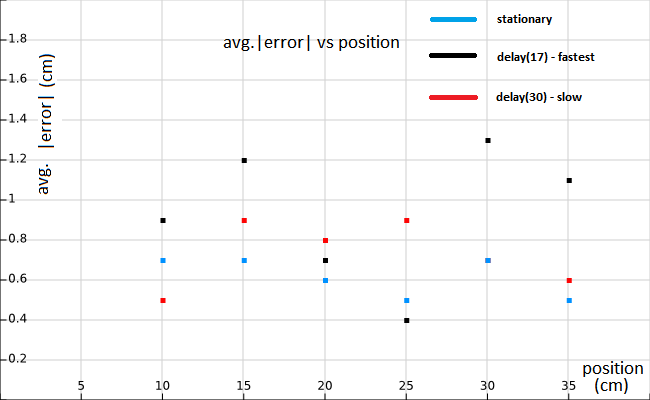
\includegraphics[width=0.8\textwidth]{../Files/save12}\\
		
		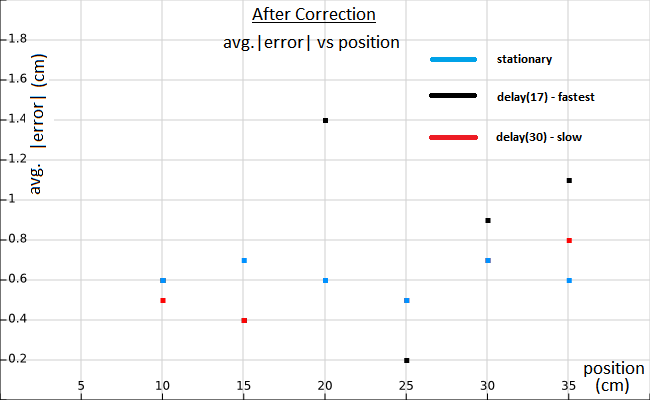
\includegraphics[width=0.8\textwidth]{../Files/save11}
		\caption{Object1-avg.|error| vs position, before vs. after correction}  
	\end{figure}
	\begin{figure}[H]
		\vfill
		\centering
		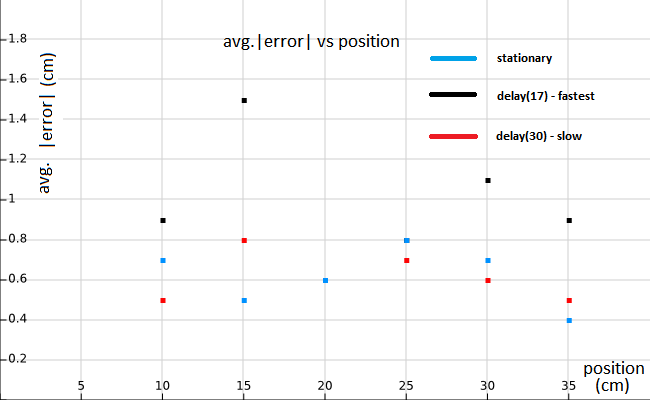
\includegraphics[width=0.8\textwidth]{../Files/save21}\\
		
		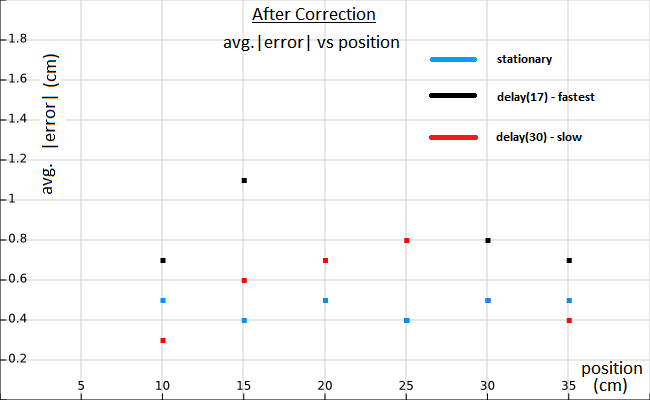
\includegraphics[width=0.8\textwidth]{../Files/save20}
		\caption{Object2-avg.|error| vs position, before vs. after correction}  
	\end{figure}
	\begin{figure}[H]
		\vfill
		\centering
		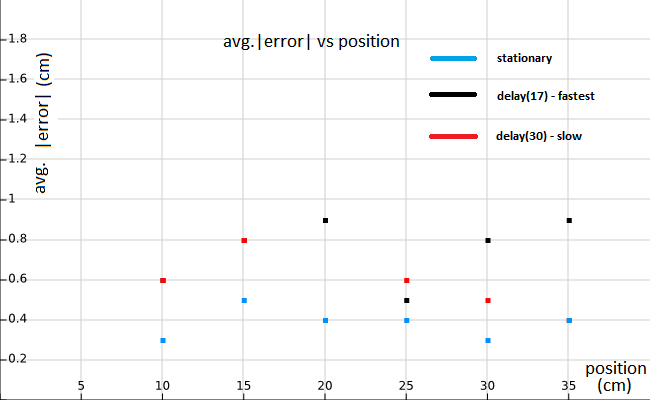
\includegraphics[width=0.8\textwidth]{../Files/save32}\\
		
		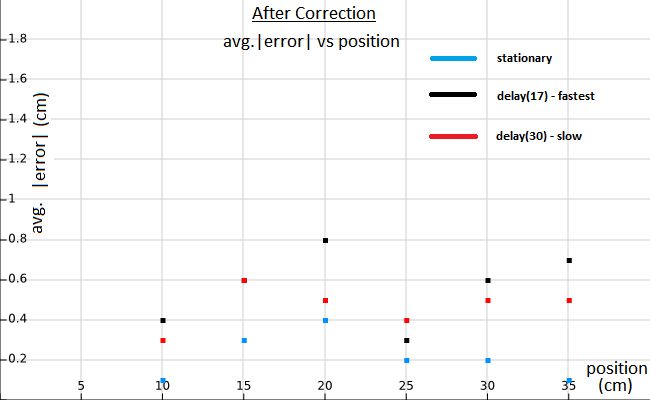
\includegraphics[width=0.8\textwidth]{../Files/save31}
		\caption{Object3-avg.|error| vs position, before vs. after correction}  
	\end{figure}
	\begin{figure}[H]
		\vfill
		\centering
		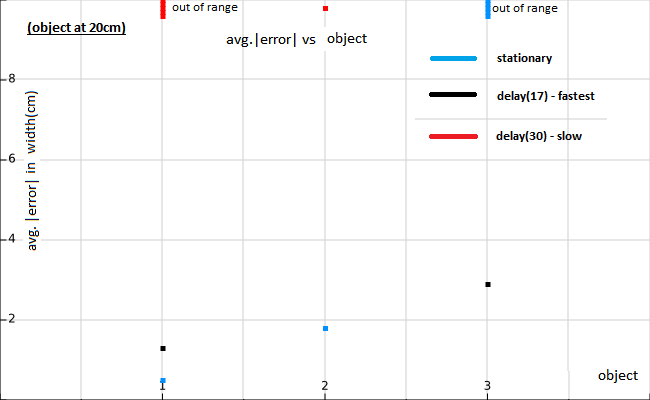
\includegraphics[width=0.8\textwidth]{../Files/savew1}\\
		
		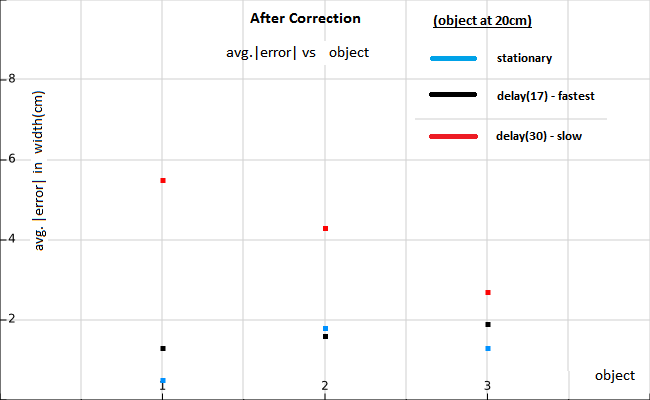
\includegraphics[width=0.8\textwidth]{../Files/savew2}
		\caption{Object-wise:avg.|error| in width at x=20cm, before vs. after correction}  
	\end{figure}
